\documentclass{article}

\textwidth=6.5in
\textheight=8.5in
\voffset=-54pt
\oddsidemargin=0in
\evensidemargin=0in
\setlength{\parskip}{8pt}
\setlength{\parindent}{0pt}

\usepackage{amsmath, amssymb}
\usepackage{ifthen}

\usepackage[inline]{enumitem}
\setlist{topsep=0pt, parsep=8pt}

\usepackage[rgb,table]{xcolor}\convertcolorsUfalse
\usepackage{graphicx}

% change hyperref options
\PassOptionsToPackage{hyphens}{url}
\usepackage[bookmarks,colorlinks,linkcolor=black,citecolor=blue,pdfstartview=FitH,urlcolor=blue]{hyperref}
\hypersetup{pdfpagemode=UseNone}
\usepackage{bookmark}

\usepackage{graphicx}
\usepackage{multicol}
\usepackage{framed}
\usepackage{array}

\usepackage{icomma}

\usepackage{soul}
\usepackage[normalem]{ulem}

\usepackage{pgfplots}
\pgfplotsset{compat=1.18}  
\pgfplotscreateplotcyclelist{mycolor}{black, blue, red, green!70!black, magenta, purple, cyan, orange }  
\pgfplotsset{
  disabledatascaling,
  cycle list=tikzcolor, 
  axis lines=middle,
  every axis plot/.style={no marks, thick},
  every axis/.style={
    enlarge x limits=false,
    enlarge y limits=auto,
    xlabel style={at={(current axis.right of origin)},anchor=west},
    ylabel style={at={(current axis.above origin)},anchor=south},
    % extra x and y ticks for asymptotes
    extra x tick style={grid=major, grid style={dashed,black}},
    extra y tick style={grid=major, grid style={dashed,black}},
    /pgf/number format/1000 sep={},
  },    
  tick label style = {font=\footnotesize, fill=\currentbgcolor, inner sep=0pt},    
  xticklabel shift=1pt,    
  scaled ticks=false,
  scaled y ticks=false,
  unbounded coords=jump,
  samples=101,
  minor tick length=0,
  scatter/classes={
    open={mark=*,draw=black,fill=white, mark size=2, thin},
    closed={mark=*,draw=black,fill=black, mark size=2, thin}
  },
  width=3in,
}
\pgfplotsset{open/.style={only marks, mark=*, fill=white, thin, mark size=2}}
\pgfplotsset{closed/.style={only marks, mark=*, draw=black, fill=black,
    thin, mark size=2}}
\pgfplotsset{labeled/.style={nodes near coords, only marks, mark=*, draw=black, fill=black, thin, mark size=2, point meta=explicit symbolic}}

\usepackage{tikz}
\usetikzlibrary{
  matrix,%
  % enables the snake paths
  decorations.pathmorphing,%
  % enables bigger arrows
  decorations.markings,%
  decorations.pathreplacing,%
  decorations.text,%
  calc,%
  patterns,%
  shapes.geometric,%
  arrows,
  decorations.shapes,
  positioning,
  plotmarks,
  intersections,
  spy
}
\tikzset{>=latex} % sets default arrow type in tikz
\tikzset{font=\normalsize}
\tikzset{mark size=1.5pt, mark options=thin}
\tikzset{pin distance=4pt,
  every pin edge/.style={<-, thin, shorten <= -2pt}}

\interfootnotelinepenalty=10000
\renewcommand{\thefootnote}{(\arabic{footnote})}

\usepackage{multirow, bigdelim}

% change to \usepackage[sols]{handout} to see solutions
\usepackage[]{handout}

\newcommand\iscurrentenumi[1]{%
  \ifthenelse{\equal{#1}{\theenumi}}{}{#1}}
\setenumerate[1]{ref=\#\arabic*}
\setenumerate[2]{ref=\protect\iscurrentenumi{\theenumi}(\alph*)}
\newcommand\enumiiprefix[2]{%
  \ifthenelse{{\equal{#1}{\theenumi}}\AND{\equal{#2}{(\alph{enumii})}}}{}{}%
  \ifthenelse{{\equal{#1}{\theenumi}}\AND{\NOT{\equal{#2}{(\alph{enumii})}}}}{#2}{}%
  \ifthenelse{\equal{#1}{\theenumi}}{}{#1#2}%
}
\setenumerate[3]{ref=\protect\enumiiprefix{\theenumi}{(\alph{enumii})}\roman*}

\makeatletter

% underline links               
\let\@href=\href
\renewcommand{\href}[2]{\@href{#1}{\ul{#2}}}

\newdimen\SOUL@dimen %new
\def\SOUL@ulunderline#1{{%
    \setbox\z@\hbox{#1}%
    % \dimen@=\wd\z@
    \SOUL@dimen=\wd\z@ %new
    \dimen@i=\SOUL@uloverlap
    \advance\SOUL@dimen2\dimen@i %\dimen@ exchanged too
    \rlap{%
      \null
      \kern-\dimen@i
      % \SOUL@ulcolor{\SOUL@ulleaders\hskip\dimen@}%
      \SOUL@ulcolor{\SOUL@ulleaders\hskip\SOUL@dimen}% new
    }%
    \unhcopy\z@
  }}

\newcommand\calculator{
  
\begin{tikzpicture}[x=0.15ex, y=0.15ex, baseline=1.5pt]
    \begin{scope}[thick]
      \draw (0, 0) -- (10, 0) -- (10, 14) -- (0, 14) -- cycle;
      \foreach \x in {10/3, 20/3}
      {
        \draw (\x, 0) -- (\x, 10);
      }
      \foreach \y in {10/3, 20/3, 10}
      {
        \draw (0, \y) -- (10, \y);
      }
    \end{scope}
  \end{tikzpicture}
}
\newcommand{\calcitem}{\refstepcounter{enum\romannumeral\@enumdepth}%
\item[\calculator \csname labelenum\romannumeral\@enumdepth\endcsname]}

\makeatother

\definecolor{purple}{rgb}{0.5,0,1.0}

\newcommand{\psreflection}[2][]{

  \ifthenelse{\not\equal{#1}{nocite}}{
    \begin{enumerate}[resume]
    \item
      \begin{problem}[1in]
        Please cite any help you got on this problem set:
        \begin{itemize}[nosep]
        \item If you worked with other students, please list their names here.
        \item If you used resources other than those on our Canvas site, please list them here.
        \end{itemize}
      \end{problem}

    \end{enumerate}
  }

  \probonly{%
    #2

    \newpage

    \emph{Reflection space.} It's a good habit to take a few minutes at the end of each pset to reflect on what you learned and jot down notes to your future self. Here are a few reflection questions to get you started. Nothing you write here will be graded; it's just for you!
    \begin{itemize}
    \item Take a few minutes to look back at the problems. How could you explain to someone else how to do each problem? What was your strategy, and how did you know to use that strategy? If there are problems where you don't feel able to answer this, write down which ones they are. Come back to them in a few days when we post the homework solutions!

      \vspace{1.5in}

    \item Take a look back at the learning objectives on today's worksheet; how are you feeling about each one? If there are ones you know you need more practice with, write those down here.

      \vspace{1.5in}

    \item What did you find most challenging about this material? Do you have any lingering questions about it? If so, write them down here so you don't forget them. At some point, stop by office hours or MQC to ask!

      \vfill
    \end{itemize}      
  }
}

\usepackage{fancyhdr}
\lhead{\textcolor{white}{This content is protected and may not be shared, uploaded, or distributed.}}
\rhead{}
\rfoot{\vspace*{\fill}\footnotesize\textcopyright{} \emph{Harvard Math Ma}}
\renewcommand{\headrulewidth}{0pt}
\pagestyle{fancy}
\begin{document}

\begin{center}
  \large\textsc{Problem Set 8 - Approximating with Secant Lines}\vspace{.5in}
  
   \large Name: \rule{5cm}{0.15mm}\\
\end{center}

\probonly{There is no Edfinity for this problem set!}

\begin{enumerate}
\item % 4.1.3

  It's 10:30 am. Over the past half hour, six customers have walked into the corner delicatessen.

  \begin{enumerate} 

  \item

    \begin{grading}
      2 points: 1 for saying 3 customers, 1 for stating that we're assuming a constant rate
    \end{grading}

    \begin{problem}[\vfill]
      How many people might the owner expect to miss if he were to close the deli to run an errand for the next 15 minutes? Upon what assumption is this based?
    \end{problem}

    \begin{solution} 
      If we assume that the average rate at which customers come to the deli is constant, he would miss $3$ customers.
    \end{solution} 

  \item

    \begin{grading}
      1 point. If they give a good reason to expect the rate to stay constant, give full credit. 
    \end{grading}

    \begin{problem}[\vfill]
      Suppose that the deli had 24 customers between 9:30 am and 11:30 am. Is it reasonable to assume that the deli will have 24 more customers between 11:30 am and 1:30 pm? Why or why not?
    \end{problem}

    \begin{solution}
      Many more customers may come around lunch time than in the morning, so this doesn't seem reasonable.
    \end{solution}

  \end{enumerate} 

\item  \begin{grading}
    1.5 points: If they pick the right value of $x$ but don't have a correct graph, deduct 1.
  \end{grading}

  \begin{problem}[\stretch{2}]
    Below is a graph $y = f(x)$. There's one value of $x$ where $f$ is \uline{not} locally linear. What value of $x$?  Sketch what the graph of $f$ looks like if you zoom in a lot around that value of $x$. 

    \begin{tikzpicture}
      \begin{axis}[width=4in, height=2.5in, xtick={-7, ..., 7}, ytick=\empty]
        \addplot+[domain=-7.7:-3] {1.5*(x+5)^2 -6 + sqrt(2)}; %
        \addplot+[domain=-3:2] {-2*sin(deg(pi*x/4))}; %
        \addplot+[domain=2:5.3] {-2}; %
      \end{axis}
    \end{tikzpicture}
  \end{problem}

  \probonly{If you're having trouble visualizing this, here's an interactive applet: \url{https://www.geogebra.org/m/wawrraj4}}

  \begin{solution}
    The function is not locally linear at $x=-3$. If we zoom in, the graph looks like this.
    \begin{tikzpicture}[spy using outlines={circle, magnification=5, connect spies}]
      \begin{axis}[width=4in, height=2.5in, xtick={-7, ..., 7}, ytick=\empty]
        \addplot+[domain=-7.7:-3] {1.5*(x+5)^2 -6 + sqrt(2)}; %
        \addplot+[domain=-3:2] {-2*sin(deg(pi*x/4))}; %
        \addplot+[domain=2:5.3] {-2}; %
        \coordinate (A) at (-3, 1.414);
        \coordinate (B) at (-5, 3);
      \end{axis}
      \spy[size=1.5cm] on (A) in node at (B); 
    \end{tikzpicture}
  \end{solution}

  \pspace{\newpage}

\item \label{secant-line-approx-sqrt(30)}

  \begin{grading}
    6 points:
    \begin{itemize}
    \item 1 for picking an appropriate secant line. The best choice is to use the secant line between $x = 25$ and $x = 36$, but we'll also accept a secant line between $x = 16$ and $x = 25$, or between $x = 36$ and $x = 49$.
    \item 1 for finding the secant line correctly. (The secant line between $x = 16$ and $x = 25$ is $y = 5 + \frac{1}{9} (x - 25) = \frac{1}{9} x + \frac{20}{9}$, and the secant line between $x = 36$ and $x = 49$ is $y = 6 + \frac{1}{13} (x - 36) = \frac{1}{13} x + \frac{42}{13}$.)
    \item 1 for correctly plugging $x = 30$ into their secant line. (If they use the secant line between $x = 16$ and $x = 25$, they should get $\frac{50}{9}$. If they use the secant line between $x = 36$ and $x = 49$, they should get $\frac{72}{13}$.)
    \item 1 for explaining whether they get an upper bound or lower bound (if they use either of the alternate choices, they'll get an upper bound)
    \item 2 points for a picture that illustrates their secant line and why it's an upper bound / lower bound
    \end{itemize}    
  \end{grading}

  \begin{problem}[\nstretch{4}]
    Sketch a graph of $f(x) = \sqrt{x}$. Use an appropriate secant
    line to approximate $\sqrt{30}$ by hand. Is your estimate an upper bound or
    lower bound for the actual value of $\sqrt{30}$? Use a picture to
    illustrate why.
  \end{problem}

  \begin{solution}
    Two points close to $(30, \sqrt{30})$ whose values we can compute are $(25, 5)$ and $(36, 6)$. The slope
    of the secant line between these two points is $\frac{6-5}{36-25}=\frac{1}{11}$. In point-slope form, the
    equation of the secant line is
    \[y-10= \frac{1}{11}(x-25),\]
    which we will rewrite as $\boxed{y=\frac{1}{11}(x-25)+5}$.
    We can plug in $x=30$ to find that
    \[
        \sqrt{30} \approx \frac{1}{11}(30-25) + 5 
        = \frac{5}{11} + 5 
        = \frac{60}{11}.
    \]

    This estimate is a lower bound for $\sqrt{30}$ because the secant line between $x=25$ and $x=36$ is below the
    graph of $y=\sqrt{x}$ at $x=30$.
   
      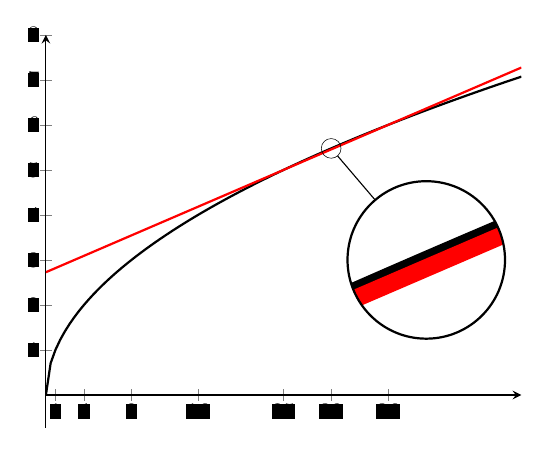
\begin{tikzpicture}[spy using outlines={circle, magnification=8, connect spies}]
        \begin{axis}[width=3in,xtick={1,4,9,16,25,30,36}, ytick distance=1]
          \addplot[domain=0:50]{sqrt(x)};
          \addplot[red, domain=0:50]{(1/11) * (x-25) + 5};
          \coordinate (A) at (30, 5.477);
          \coordinate (B) at (40,3);
        \end{axis}
        \spy[size=2cm] on (A) in node at (B);
      \end{tikzpicture}

    
      
  \end{solution}

\calcitem \label{usain-bolt} 

  At the 2008 Olympics in Beijing, sprinter Usain Bolt of Jamaica broke
  the world record for the $100$ meters.  Bolt's times for every ten
  meters of the race were as follows: % from http://speedendurance.com/2008/08/22/usain-bolt-100m-10-meter-splits-and-speed-endurance/
  \begin{center}
    \begin{tabular}{l*{10}{c}}
      \hline
      Distance (meters) & $10$ &  $20$ &  $30$ &  $40$ &  $50$ &
      $60$ &  $70$ &  $80$ &  $90$ &  $100$ \\
      \hline
      Time (seconds) & $1.85$ & $2.87$ &  $3.78$ & $4.65$ &  $5.50$ &
      $6.32$ & $7.14$ & $7.96$ & $8.79$ & $9.69$ \\
      \hline
    \end{tabular}
  \end{center}

  \begin{enumerate}
  \item

    \begin{grading}
      1 point: 0.5 for calculation, 0.5 for units
    \end{grading}

    \begin{problem}[\vfill] \label{bolt-2008-total}
      What was Bolt's average speed for the entire race? Please
      include units. 
    \end{problem}

    \begin{solution} % Jason Bland
      average speed = $\dfrac{\text{distance}}{\text{time}} = \dfrac{100
        \text{ m}}{9.69 \text{ s}} \approx 10.32$ meters per second
    \end{solution}

  \item \label{bolt-2008-first-50}

    \begin{grading}
      1 point
    \end{grading}

    \begin{problem}[\vfill]
      What was Bolt's average speed for the first 50 meters of the race?
    \end{problem}

    \begin{solution} % Jason Bland
      $\dfrac{50 \text{ m}}{5.50 \text{ s}} \approx 9.09$ meters per
      second 
    \end{solution}

  \item \label{bolt-2008-last-50}

    \begin{grading}
      1 point
    \end{grading}

    \begin{problem}[\vfill]
      What was Bolt's average speed for the last 50 meters of the race?
    \end{problem}

    \begin{solution} % Jason Bland
      The last 50 meters of the race took Bolt $9.69 - 5.50 = 4.19$
      seconds, so his average speed was $\dfrac{50 \text{ m}}{4.19 \text{
          s}} \approx 11.93$ meters per second.
    \end{solution}

  \item

    \begin{grading}
      1 point
    \end{grading}

    \begin{problem}[\stretch{1.25}]
      If you average your answers to \ref{bolt-2008-first-50} and
      \ref{bolt-2008-last-50}, do you get Bolt's average speed for the
      entire race?
    \end{problem}

    \begin{solution} % Jason Bland
      No. Averaging the answers to \ref{bolt-2008-first-50} and
      \ref{bolt-2008-last-50} gives $\approx \dfrac{9.09 + 11.93}{2} =
      10.51$ meters per second, which is not the same as our answer to
      \ref{bolt-2008-total}. We've seen in
      \href{https://people.math.harvard.edu/~jjchen/mathma/docs/homework/PS03.html}{Problem Set 3}, {{{{\#5}}(c)}} why this is.
    \end{solution}

  \item

    \begin{grading}
      2 points: 1 for correct intervals, 1 for reasoning
    \end{grading}

    \begin{problem}[\nstretch{4}]
      Over which 10-meter interval(s) (0 to 10 m, 10 to 20 m, 20 to 30 m, etc.)\ was Bolt's average speed the highest during this race? Explain your reasoning.
    \end{problem}

    \begin{solution} % Jason Bland
      Since average speed is $\frac{\text{distance}}{\text{time}}$ and we're looking at intervals where the distance is 10 m, his average speed is highest when the time taken is lowest. Here are the times spent in each interval:
      \begin{center}
        \begin{tabular}{l*{5}{c}}
          \hline
          Interval (meters) & $0$ to $10$ &  $10$ to $20$ &  $20$ to $30$ &  $30$ to $40$ &  $40$ to $50$ \\
          \hline
          Time (seconds) & $1.85$ & $1.02$ &  $0.91$ & $0.87$ &  $0.85$ \\
          \hline \hline
          Interval (meters) & $50$ to $60$ &  $60$ to $70$ &  $70$ to $80$ &  $80$ to $90$ &  $90$ to $100$ \\
          \hline
          Time (seconds) & $0.82$ & $0.82$ & $0.82$ & $0.83$ & $0.90$ \\
          \hline
        \end{tabular}
      \end{center}
      So, his average speed is tied for highest among the intervals \fbox{50 to 60 meters}, \fbox{60 to 70 meters}, and \fbox{70 to 80 meters}.
    \end{solution}

  \item
    \begin{grading}
      1 point
    \end{grading}

    \begin{problem}[\vfill]
      To observers, Bolt appeared to slow down toward the end of the race
      to celebrate his victory.  Does the data support this observation?
      Explain. 
    \end{problem}

    \begin{solution} % Jason Bland
      Yes. The time spent during the last 10 meters was more than in each
      of the previous six 10 meter intervals. 
    \end{solution}

  \end{enumerate}

  In August 2009, Bolt set a new world record in the 100 meter dash. Bolt's times for every ten meters of this race were as follows: % https://web.archive.org/web/20140421051106/https://berlin.iaaf.org/mm/document/development/research/05/31/54/20090817073528_httppostedfile_analysis100mmenfinal_bolt_13666.pdf
  \begin{center}
    \begin{tabular}{l*{10}{c}}
      \hline
      Distance (meters) & $10$ &  $20$ &  $30$ &  $40$ &  $50$ &
      $60$ &  $70$ &  $80$ &  $90$ &  $100$ \\
      \hline
      Time (seconds) & $1.89$ & $2.88$ &  $3.78$ & $4.64$ &  $5.47$ &
      $6.29$ & $7.10$ & $7.92$ & $8.75$ & $9.58$ \\
      \hline
    \end{tabular}
  \end{center}
  \begin{enumerate}[resume]
  \item

    \begin{grading}
      1 point
    \end{grading}

    \begin{problem}[\vfill]
      Analysts noted that Bolt reached his top speed $65$ meters into the
      race.  Use the data above to estimate this speed.
    \end{problem}

    \begin{solution} % Jason Bland
      We can estimate Bolt's speed 65 meters into the race as
      approximately his average speed between 60 meters and 70 meters,
      which is $\dfrac{10 \text{ m}}{7.10-6.29 \text{ s}} \approx 12.35$
      meters per second.
    \end{solution}

  \item
    \begin{grading}
      2 points. 
    \end{grading}

    \begin{problem}[\vfill]
      Did Bolt slow down toward the end of this race, as he did in the 2008 Olympics?
    \end{problem}

    \begin{solution} % Jason Bland
      Again, we can look at the time taken for each 10 m interval:
      \begin{center}
        \begin{tabular}{l*{5}{c}}
          \hline
          Interval (meters) & $0$ to $10$ &  $10$ to $20$ &  $20$ to $30$ &  $30$ to $40$ &  $40$ to $50$ \\
          \hline
          Time (seconds) & 1.89 & 0.99 & 0.9 & 0.86 & 0.83 \\
          \hline \hline
          Interval (meters) & $50$ to $60$ &  $60$ to $70$ &  $70$ to $80$ &  $80$ to $90$ &  $90$ to $100$ \\
          \hline
          Time (seconds) & 0.82 & 0.81 & 0.82 & 0.83 & 0.83 \\
          \hline
        \end{tabular}
      \end{center}
      The last 10 m did not take much longer than the previous few 10 m
      intervals, so he did not slow down significantly. 
    \end{solution}

  \item

    \begin{grading}
      2 points. They don't have to give exactly the same estimate as the solution; just look for correct reasoning and methodology. 
    \end{grading}

    \begin{problem}[\nstretch{2}]
      Estimate what Bolt's time in the 2008 Olympics could have been if he hadn't slowed down to celebrate. Explain how you obtain your estimate.
    \end{problem}

    \begin{solution}
      As we can see from the 2009 race, Bolt can run the last 10 m in the
      same amount of time as the previous 10 m; thus, a reasonable
      assumption is that, in 2008, he could have run the last 10 m in
      $0.83$ seconds.  This would have been $0.07$ seconds faster than
      what he actually did, for a total of $9.62$ seconds.
    \end{solution}

  \end{enumerate}

\calcitem \label{sea-ice-when-ice-free} 

  Let's look again at the \href{https://docs.google.com/spreadsheets/d/1Dx8q2itdxCfEfRMkhUi4188zXYFqXQ2MB1_svnefxyg/edit?usp=sharing}{data about the minimum extent of Arctic sea ice each year} that you looked at in \href{https://canvas.harvard.edu/files/20663280/download?download_frd=1}{Problem Set 3}, {{\#3}}.

  As \href{https://www.nytimes.com/2023/06/06/climate/arctic-sea-ice-melting.html?unlocked_article_code=1.HU4.c_XS.kUPtWv2pzsvT&smid=url-share}{this article} explains, ``Over the course of every year, the surface water of the Arctic Ocean freezes and melts with the seasons. The amount of ice grows in winter, peaks around March, then declines toward an annual minimum, typically in September.

  The September lows have been edging downward ever since continuous satellite measurements began in 1979, leading researchers to try to predict when the ocean might experience its first summer that melts effectively all of the floating ice.''

  In this problem, you'll make such a prediction and analyze it.

  \begin{enumerate}
  \item

    \begin{grading}
      2 points: 1 for slope, 1 for equation
    \end{grading}

    \begin{problem}[\vfill]
      As you saw in \href{https://canvas.harvard.edu/files/20663280/download?download_frd=1}{Problem Set 3}, {{\#3}}, the average rate of change of this data between 1979 and 2022 seems slightly different from the overall trend. The trend seems better described by the average rate of change between 1982 and 2009.\probonly{\footnote{If you go on to take more quantitative courses, you'll probably learn how to find a ``best-fit line'', which is a line that is ``closest'' to data points in a particular way. We won't get to this idea in Math M, but the best-fit line for this data is very close to the secant line between 1982 and 2009.}}

      Use the \href{https://docs.google.com/spreadsheets/d/1Dx8q2itdxCfEfRMkhUi4188zXYFqXQ2MB1_svnefxyg/edit?usp=sharing}{data in the spreadsheet} to find the equation of the secant line between 1982 and 2009.
    \end{problem}

    \begin{solution}
      In 1982, the annual minimum sea ice extent was 7.166 million square kilometers, and in 2009, it was 5.119 million
      square kilometers.

      The average rate of change between 1982 and 2009 is
      \[\frac{5.119-7.166}{2009-1982}\approx -0.0758\text{ million km$^2$ per year}.\]

      This is the slope of the secant line, and we can use point-slope form to write the equation:
      \[\boxed{y - 5.119 = -0.0758(x-2009).}\]
    \end{solution}

  \item \label{sea-ice-when-ice-free-secant-line-prediction}

    \begin{grading}
      2 points: 1 for knowing to solve for where the $y$-value of the line is 1 million km$^2$, 1 for carrying this out correctly 
    \end{grading}

    \begin{problem}[\vfill\newpage]
      The threshold scientists use for declaring the Arctic ``practically ice-free'' is having less than 1 million km$^2$ of ice. Use your secant line to predict the year in which the annual minimum sea ice extent will first drop below 1 million km$^2$.
    \end{problem}

    \begin{solution}
      We can substitute $y=1$ in the equation of the secant line and solve for $x$:
      \begin{align*}
        1 - 5.119 &= -0.0758(x-2009) \\
        54.34 &= x-2009 \\
        x & \approx 2063.
      \end{align*}
      Using the secant line between 1982 and 2009, we predict that the first year in which the Arctic will be
      ``practically ice-free'' will be \fbox{2063}.
    \end{solution}

  \item \label{sea-ice-compare-prediction}

    \begin{grading}
      1 point  
    \end{grading}

    \begin{problem}[\stretch{0.5}]
      \href{https://www.nytimes.com/2023/06/06/climate/arctic-sea-ice-melting.html?unlocked_article_code=1.HU4.c_XS.kUPtWv2pzsvT&smid=url-share}{The article} goes on to explain that \href{https://www.nature.com/articles/s41467-023-38511-8}{a new study} predicts that the Arctic will be practically ice-free as early as the 2030s. How does this compare to your secant line prediction?
    \end{problem}

    \begin{solution}
      The study's prediction is much earlier than our secant line prediction.
    \end{solution}

  \item

    \begin{grading}
      3 points: 1 for recognizing that we're assuming the rate is constant, 1 for recognizing the assumption must not be valid, 1 for including a supporting quote 
    \end{grading}

    \begin{problem}[\vfill]
      What assumption are we making in \ref{sea-ice-when-ice-free-secant-line-prediction} when we use the secant line to make this prediction? What does \ref{sea-ice-compare-prediction} suggest about the validity of this assumption? Read through \href{https://www.nytimes.com/2023/06/06/climate/arctic-sea-ice-melting.html?unlocked_article_code=1.HU4.c_XS.kUPtWv2pzsvT&smid=url-share}{the article} again, and write down at least one quote from the article that supports your view of how valid the assumption is.
    \end{problem}

    \begin{solution}
      In part (b), we are assuming that the rate of change of the annual minimum sea ice extent with respect to 
      time will remain constant. Based on the results of the study, this assumption is not valid. 
      
      Relevant quotes:
        \begin{quote}
          ``Sea ice reflects solar radiation back into space, so the less ice there is, the faster the Arctic warms. This causes the Greenland ice sheet to melt more quickly, adding to sea-level rise globally.''
        \end{quote}
        \begin{quote}
          ``Our result suggests that the Arctic amplification will be coming faster and stronger,'' said Seung-Ki Min, a climate scientist at Pohang University of Science and Technology in South Korea and another author of the new paper. ``That means the related impacts will be also coming faster.''
        \end{quote}
    \end{solution}

    


  \end{enumerate}

\item  \begin{grading}
    3.5 points: 1 for knowing the slope is $\dfrac{ f(3+k) - f(3) }{k}$, 0.5 for correctly using the formula for $f$, 2 for correctly simplifying completely. (If they simplify partially, give them part of this 2.)
  \end{grading}

  \begin{problem}[\nstretch{2.5}]
    Let $f(x) = \frac{3}{x} + 2x$. Find the slope of the secant line through the points with $x = 3$ and $x = 3 + k$, where $k \neq 0$. Simplify your answer completely.
  \end{problem}

  \begin{solution}
    The slope of the secant line is 
    \begin{align*} 
      \frac{ f(3+k) - f(3) }{3+k - 3}  &=  \frac{\frac{  3}{3+k} +2
        (3+k) - \left( \frac{3}{3} + 6 \right)}{k} \\
      &= \frac{\frac{  3}{3+k} +2k - 1}{k} \\
      \intertext{To get rid of the denominator $3 + k$ in the
        numerator, let's strategically multiply this by 1 (which
        doesn't change the expression):}
      &= \frac{\frac{  3}{3+k} +2k - 1}{k} \cdot \frac{3 + k}{3 + k}
      \\
      &= \frac{3 + 2k (3 + k) - (3 + k)}{k (3 + k)} \\
      &= \frac{2k^2 + 5k}{k (3 + k)} \\
      &= \frac{k (2k + 5)}{k (3 + k)} \\
      \intertext{Since $k \neq 0$, we can cancel the $k$ in the numerator and the $k$ in the denominator:} %
      & =  \boxed{ \frac{  2 k + 5}{3+k} }
    \end{align*}  
  \end{solution}

\item 

  \begin{grading}
    3 points. Any thoughtful response gets full credit. 
  \end{grading}

  \begin{problem}[\vfill]
    There are many stereotypes about people who use math in their careers. In reality, all sorts of people do math, and each person has had a different journey.

    Pick one of the following to read or watch; write down which one you chose and your reaction to it. Did you find anything particularly interesting about the person's path? Surprising? Relatable?
    \begin{itemize}
    \item John Urschel is a mathematician who got his PhD at MIT while playing football for the Baltimore Ravens. Watch this \href{https://www.youtube.com/watch?v=Hp20Z0QyKJE}{video} where he shares his journey.
    \item Barbara Oakley is an engineering professor who hated math and science all through high school and her early career in the army. In \href{https://canvas.harvard.edu/files/20608918/download?download_frd=1}{this excerpt} from her book \href{https://barbaraoakley.com/books/a-mind-for-numbers/}{\emph{A Mind for Numbers}}, she shares her story.
    \item Vanessa Vakharia started a math and science tutoring studio; in \href{https://www.youtube.com/watch?v=hI-c1bCUc8A}{this video}, she talks about her journey since failing math twice in 11th grade.
    \item The book \href{https://canvas.harvard.edu/files/20608917/download?download_frd=1}{\emph{Living Proof}} is a collection of stories by accomplished mathematicians about challenges they've faced. Pick any chapter to read. 
    \end{itemize}
  \end{problem}

\end{enumerate}
\psreflection{For next class, read \S 5.1, 5.4.}
\end{document}
